\subsection{Flip-Flop JK}

O flip-flop JK é uma evolução do latch SR que resolve o estado inválido.

Entradas:
\begin{itemize}
    \item $J$ (Set)
    \item $K$ (Reset)
\end{itemize}

Tabela de transição:

\begin{center}
\begin{tabular}{c c | c}
J & K & $Q_{t+1}$ \\
\hline
0 & 0 & $Q_t$ \\
0 & 1 & 0 \\
1 & 0 & 1 \\
1 & 1 & $\overline{Q_t}$
\end{tabular}
\end{center}

A pode ser feita da seguite forma: 

\begin{figure}[H]
    \centering
    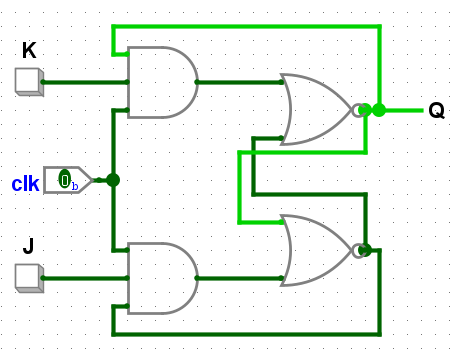
\includegraphics[width=0.6\linewidth]{images/JK-FF-circuit.png}
    \caption{Implementação do Flip Flop JK a partir do SR Nor Latch no Logisim Evolution}
    \label{fig:JK-FF-circuit}
\end{figure}

\begin{figure}[H]
    \centering
    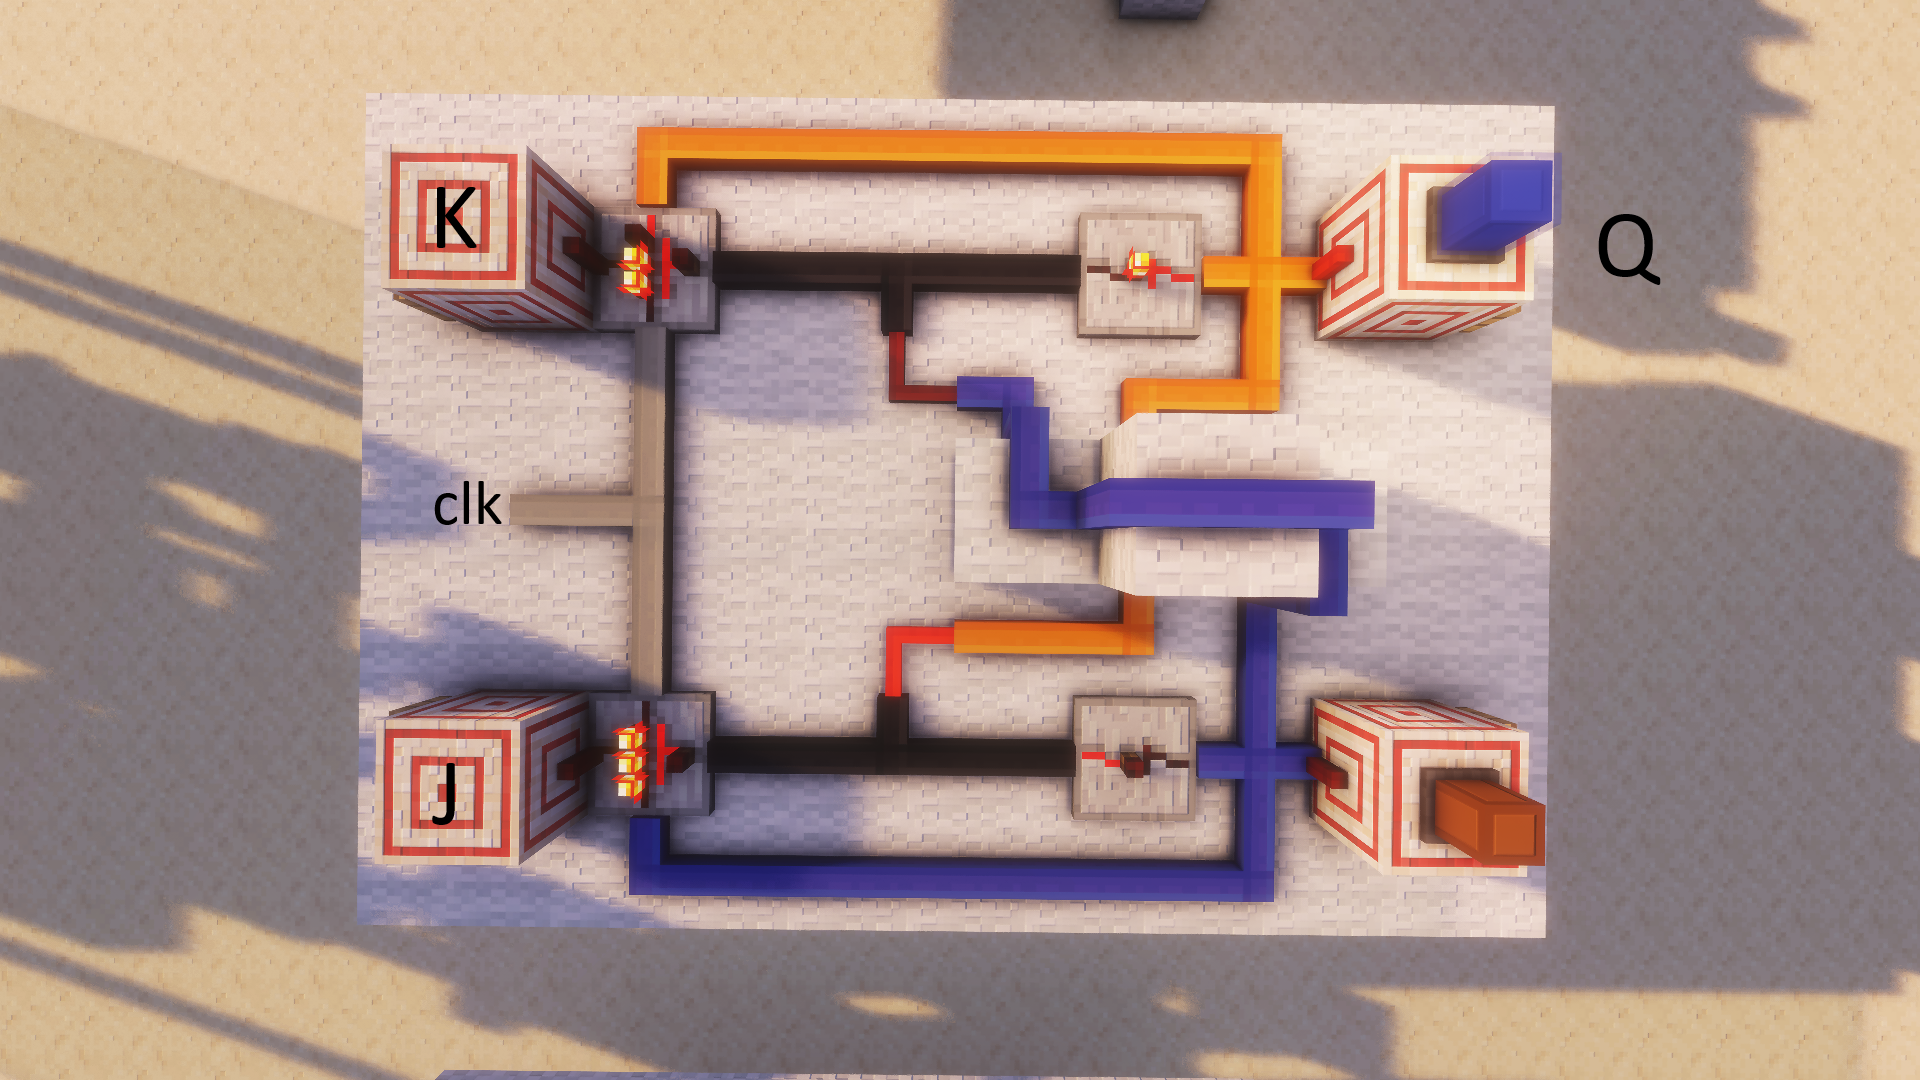
\includegraphics[width=0.8\linewidth]{images/JK-FF-redstone.png}
    \caption{Implementação do Flip Flop JK a partir do SR Nor Latch no Minecraft}
    \label{fig:JK-FF-redstone}
\end{figure}

O estado $Q$ é atualizado apenas durante o nível ativo do sinal de clock. No entanto, quando $J = K = 1$, o circuito tende a alternar continuamente entre $Q$ e $\lnot Q$ devido à realimentação interna.

Para evitar esse comportamento, é necessário que a duração do pulso de clock ($t_{high}$) seja menor que o tempo total de propagação do circuito ($t_{loop}$):

\[
t_{high} < t_{loop}
\]

Nesse contexto, detectores de borda podem ser utilizados para transformar o sinal de clock em pulsos extremamente curtos, associados apenas às transições do sinal.

Dessa forma, garante-se que apenas uma transição de estado ocorra por pulso de clock, evitando múltiplas comutações indesejadas.

Esse problema é conhecido como \textit{race-around condition} e ocorre em implementações sensíveis ao nível do clock.